% --------------------- NO TOCAR ----------------------
\documentclass[a4paper, 10pt, twocolumn]{report}
\input plantillaTeXpracticasRL.sty % Incluir fichero de estilo del máster
% -----------------------------------------------------



% MODIFICA ESTOS DATOS
% Incluir el nombre de la obra y los nombres completos de los autores del trabajo, junto con el correo electrónico um.es para cada autor.
\title{Aprendizaje por Refuerzo}
\author{
Guillermo Carmona Martínez 	\\
\texttt{
g.carmonamartinez@um.es} \\[0.25cm]
Francisco José Cortes Delgado 	\\
\texttt{
franciscojose.cortesd@um.es} \\[0.25cm]
Víctor Saura Meseguer 	\\
\texttt{victor.sauram@um.es}}



\begin{document}

% Carátula
\maketitle % Puedes modificar la carátula usando el entorno titlepage.

% Resumen
% --------------------- NO TOCAR ----------------------
\renewcommand{\abstractname}{Resumen}
% -----------------------------------------------------

% HAZ UN RESUMEN DE TU TRABAJO. ES UN RESUMEN, NO ES UNA INTRODUCCIÓN
\begin{abstract}    
    En este documento se presentará uno de los trabajos que puede realizar como proyecto final y que deberán de ser expuestos en público.
    
     Recuerde que la experimentación deberá de estar en un repositorio GitHub para poder contrastar lo que aquí explique. En el GitHub puede añadir tantos \textit{notebooks} como considere. Pero aquí, el trabajo documental, ocupará 10 páginas descontadas la portada, el resumen, el índice y la bibliografía.
    
    El contenido del repositorio y este documento deberán subirse al AV como evidencias del trabajo realizado.
    
    Respete las dobles columnas. Si las suprime generará un documento que ocupará más páginas. Con las dobles columnas puede incluir más contenido.
 \end{abstract}

% Índice
\begingroup
\renewcommand{\thispagestyle}[1]{}  % evitar que \chapter* sobreescriba el estilo
\pagestyle{empty}
\tableofcontents
\endgroup
\setcounter{page}{1}

% Trabajos
% MODIFICA EL CONTENIDO QUE VIENE A CONTINUACIÓN DE ACUERDO A TU TRABAJO

\chapter{Problema del Bandido de $k$-brazos}

%%%%%%%%%%%%%%%%%%%%%%%%%%%%%%%%%%%%%%%%%%%%%%%%%%%%%%%%%%%%%
%%%%%%%%%%%%%%%%%%%%%%%%%%%%%%%%%%%%%%%%%%%%%%%%%%%%%%%%%%%%%
\section{Introducción}

    %\begin{itemize}
    %    \item Breve descripción del problemas y su relevancia.
    %    \item Motivación del trabajo: ¿Por qué es importante el problema estudiado?
    %    \item Objetivos del informe: ¿Qué se pretende lograr con el desarrollo del trabajo?
    %    \item Organización del documento: breve explicación de la estructura del informe.
    %\end{itemize}

    El problema del bandido de $K$ brazos describe un escenario en el cual un agente debe elegir repetidamente entre $k$ opciones diferentes. Al seleccionar una acción, el agente recibe una recompensa numérica proveniente de una distribución de probabilidad desconocida (ej, normal, binomial, bernoulli, etc.) asociada a ese brazo. El objetivo fundamental es maximizar la recompensa total acumulada a lo largo de un número determinado de pasos de tiempo, lo que requiere que el agente aprenda qué acciones son las mejores basándose únicamente en la retroalimentación de sus decisiones previas.

    La importancia y relevancia de este problema reside en su capacidad para modelar el dilema fundamental entre \textbf{exploración} y \textbf{explotación}. Un equilibrio inadecuado entre ambas estrategias resulta costoso, ya que centrarse solo en la explotación puede ignorar la mejor opción de forma permanente, mientras que una exploración excesiva genera un alto arrepentimiento acumulado al desperdiciar recursos en opciones subóptimas. Debido a esta capacidad para optimizar decisiones bajo incertidumbre, el modelo es muy útil y práctico en aplicaciones del mundo real, como pueden ser ensayos clínicos médicos, marketing digital (pruebas A/B), sistemas de recomendación y gestión de redes.

    El objetivo de este informe es analizar y comparar las principales estrategias algorítmicas diseñadas para resolver el problema del bandido multibrazo, desde métodos básicos basados en estimaciones de valor de acción como el algoritmo el $\varepsilon$-\textit{greedy}, hasta enfoques más sofisticados como los métodos de límite superior de confianza (UCB), el ascenso del gradiente y los métodos bayesianos. En última instancia, se busca comprender cómo estas estrategias gestionan el equilibrio exploración-explotación para maximizar la recompensa obtenida en entornos inciertos. 

    El informe se organiza del siguiente modo, la sección de Desarrollo presenta la definición formal del problema, revisa los enfoques existentes en la literatura y describe los métodos implementados. La sección de Algoritmos recoge todos los algoritmos implementados, explicandolos paso a paso y mostrando su pseudocodigo. La sección de Resultados recoge los experimentos realizados y analiza el comportamiento de cada algoritmo. Finalmente, la sección de Conclusiones resume los hallazgos principales.


\section{Desarrollo}
	%\begin{itemize}
        %\item Definición formal del problema o aplicación específica abordada.
        %\item Describir enfoques existentes en la literatura sobre problemas similares.
        %\item Contexto y antecedentes necesarios para entender el trabajo.
        %\item Explicación de los métodos utilizados para abordar el problema.
        %\item Justificar cómo el presente trabajo se diferencia o mejora enfoques previos.
    %\end{itemize}

El bandido de $K$-brazos \cite{robbins1952} es un proceso de decisión secuencial en el que, en cada instante $t = 1,2,\dots,T$, un agente elige una acción $a_t \in \mathcal{A} = \{a_1,\dots,a_k\}$ y recibe una recompensa $r_t \sim p(r \mid a_t)$ proveniente de una distribución desconocida.

\begin{definition}[Valor de una acción]
El valor real de una acción $a$ es la recompensa esperada al seleccionarla: $q(a) = \mathbb{E}[R_t \mid A_t = a]$.
\end{definition}

Como $q(a)$ es desconocido, el agente debe estimarlo a partir de la experiencia. El objetivo es maximizar la recompensa acumulada $\sum_{t=1}^{T} r_t$, lo que equivale a minimizar el \textit{arrepentimiento esperado}:
\begin{equation}
    \mathbb{E}[R_T] = T\,q^* - \sum_{t=1}^{T} \mathbb{E}[r_t], \qquad q^* = \max_{a \in \mathcal{A}} q(a)
\end{equation}
El reto central es el equilibrio entre \textbf{exploración} (probar brazos poco conocidos para mejorar las estimaciones) y \textbf{explotación} (seleccionar el brazo con mayor recompensa esperada conocida).

Desde su formulación, han surgido cuatro grandes familias de soluciones para este problema:

\begin{enumerate}

    \item \textbf{Métodos acción-valor con exploración heurística.} Estiman $q(a)$ como el promedio de recompensas observadas y aplican una política que intercala explotación y exploración. El \textbf{$\varepsilon$-\textit{greedy}} explora al azar con probabilidad fija $\varepsilon$ \cite{sutton2018}, mientras que el \textbf{$\varepsilon$-decaimiento} reduce $\varepsilon$ gradualmente para favorecer la explotación conforme avanza el aprendizaje.

    \item \textbf{Métodos de índice (\textit{Upper Confidence Bound}, UCB).} Seleccionan la acción que maximiza un índice que combina valor estimado e incertidumbre. UCB1 \cite{auer2002} aplica el principio de \textit{optimismo ante la incertidumbre} y garantiza un arrepentimiento acotado por $O(\ln T)$.

    \item \textbf{Métodos de ascenso del gradiente.} Aprenden una preferencia $H_t(a)$ mediante gradiente estocástico y asignan probabilidades de selección mediante una función \textit{softmax} \cite{sutton2018}.

    \item \textbf{Métodos bayesianos.} Mantienen una distribución posterior sobre los parámetros de cada brazo, actualizada con la regla de Bayes. El \textbf{Muestreo de Thompson} \cite{thompson1933, russo2018} muestrea de la posterior y selecciona el brazo con mayor valor estimado, logrando una exploración adaptativa eficaz.

\end{enumerate}

También hay que mencionar una diferencia entre el aprendizaje supervisado, que proporciona \textbf{retroalimentación instructiva} (la acción correcta es conocida), y el bandido multibrazo, el cual opera con \textbf{retroalimentación evaluativa}. En el problema del bandido el agente solo conoce la calidad de la acción tomada, no si existía una mejor \cite{sutton2018}. Además, es un entorno \textbf{no asociativo}, pues el agente no observa ningún estado que condicione su decisión, lo que lo convierte en el modelo más simple del aprendizaje por refuerzo. A lo largo de este trabajo se asume que las distribuciones de recompensa son \textbf{estacionarias} ($p(r \mid a)$ no varía con el tiempo), condición bajo la que los algoritmos presentados ofrecen sus mejores garantías teóricas.

Se han implementado cinco algoritmos que cubren tres de las familias descritas anteriormente. Todos estiman los valores de acción mediante actualización incremental del promedio y se diferencian en su política de selección de brazos, \textbf{$\varepsilon$-Greedy}, que explora aleatoriamente con probabilidad fija $\varepsilon$. \textbf{$\varepsilon$-Greedy con inicialización}, variante que garantiza visitar todos los brazos antes de aplicar la política, corrigiendo el comportamiento incorrecto del greedy puro ($\varepsilon = 0$). \textbf{$\varepsilon$-Decaimiento}, que reduce $\varepsilon$ inversamente proporcional al tiempo para favorecer la explotación conforme avanza el aprendizaje. \textbf{UCB1} \cite{auer2002}, que selecciona el brazo con mayor límite superior de confianza combinando valor estimado e incertidumbre. Y \textbf{Softmax (Gibbs)}, que muestrea acciones según una distribución proporcional a sus valores estimados, controlada por una temperatura $\tau$. Los detalles de cada algoritmo se desarrollan en profundidad en la sección de Algoritmos. Esta selección cubre una progresión natural de complejidad que permite comparar, bajo condiciones experimentales idénticas, estrategias heurísticas simples, el enfoque con garantías teóricas de UCB1 y la política probabilística continua de Softmax.


%%%%%%%%%%%%%%%%%%%%%%%%%%%%%%%%%%%%%%%%%%%%%%%%%%%%%%%%%%%%%
%\subsection{Trabajos Relacionados}

%Por supuesto puede añadir más subapartados si los necesitara.

%%%%%%%%%%%%%%%%%%%%%%%%%%%%%%%%%%%%%%%%%%%%%%%%%%%%%%%%%%%%%
%\subsubsection{Más subsecciones}

%Pero no debería poner más de profundidad tres.

%¡Ah! No olvide poner las correspondientes citas como \cite{ref1, ref2}.



%%%%%%%%%%%%%%%%%%%%%%%%%%%%%%%%%%%%%%%%%%%%%%%%%%%%%%%%%%%%%
%%%%%%%%%%%%%%%%%%%%%%%%%%%%%%%%%%%%%%%%%%%%%%%%%%%%%%%%%%%%%
\section{Algoritmos}
    %\begin{itemize}
        %\item Explicar en detalle los pasos de los algoritmos empleados.
        %\item Incluir pseudocódigo y, opcionalmente, diagramas de flujo si es necesario.
        %\item Justificar la elección de los algoritmos y su aplicabilidad al problema estudiado.
    %\end{itemize}

A continuación se describe en detalle cada uno de los cinco algoritmos. Todos comparten la regla de actualización incremental del promedio (Algoritmo~\ref{algo:update}), que opera en tiempo y espacio $O(1)$ por paso, garantizando condiciones de comparación homogéneas. Los métodos de gradiente y bayesianos, aunque más potentes, quedan fuera del alcance de este trabajo.

\begin{algorithm}
\caption{Actualización incremental del valor estimado}\label{algo:update}
\begin{algorithmic}[1]
\Require Brazo seleccionado $a$, recompensa observada $r$
\State $N(a) \gets N(a) + 1$
\State $Q(a) \gets Q(a) + \dfrac{1}{N(a)}\bigl(r - Q(a)\bigr)$
\end{algorithmic}
\end{algorithm}

\subsection*{$\varepsilon$-Greedy}

Método más simple para incorporar exploración. Con probabilidad $\varepsilon$ selecciona un brazo aleatorio, con probabilidad $1-\varepsilon$ explota el brazo de mayor valor estimado. Los empates se rompen aleatoriamente para evitar sesgo hacia índices bajos. Es el punto de partida natural para entender el dilema exploración-explotación. Nótese que para $\varepsilon=0$ (greedy puro) el agente explota desde el primer paso sin haber visitado todos los brazos, limitación que corrige el algoritmo siguiente. Su simplicidad lo convierte en la linea base a implementar ya que cualquier mejora sobre él cuantifica directamente el beneficio de estrategias más sofisticadas.

\begin{algorithm}
\caption{$\varepsilon$-Greedy}\label{algo:egreedy}
\begin{algorithmic}[1]
\Require $k$ (brazos), $\varepsilon \in [0,1]$
\State $N(a) \gets 0$, $Q(a) \gets 0$ \textbf{para todo} $a$
\For{$t = 1, 2, \dots, T$}
    \If{$\text{Uniforme}(0,1) < \varepsilon$}
        \State $A_t \gets$ brazo aleatorio de $\{1,\dots,k\}$ \Comment{Exploración}
    \Else
        \State $A_t \gets \arg\max_a Q(a)$, empates rotos aleatoriamente \Comment{Explotación}
    \EndIf
    \State Recibir recompensa $R_t$
    \State Actualizar $N(A_t)$ y $Q(A_t)$ (Alg.~\ref{algo:update})
\EndFor
\end{algorithmic}
\end{algorithm}

\subsection*{$\varepsilon$-Greedy con inicialización}

Extiende el anterior añadiendo una fase de arranque que visita todos los brazos al menos una vez antes de aplicar la política. Esto es imprescindible para el caso $\varepsilon=0$ (greedy puro), donde sin inicialización el agente nunca exploraría. Garantiza que $Q(a)$ se basa en al menos una observación real de cada brazo antes de tomar decisiones de explotación, haciendo la comparación con $\epsilon$-Greedy más equitativa.

\begin{algorithm}
\caption{$\varepsilon$-Greedy con inicialización}\label{algo:egreedy_init}
\begin{algorithmic}[1]
\Require $k$, $\varepsilon \in [0,1]$
\State $N(a) \gets 0$, $Q(a) \gets 0$ \textbf{para todo} $a$
\For{$t = 1, 2, \dots, T$}
    \If{$\exists\, a : N(a) = 0$}
        \State $A_t \gets$ brazo aleatorio de $\{a : N(a) = 0\}$ \Comment{Inicialización}
    \EndIf
    \State Igual que Alg.~\ref{algo:egreedy}
\EndFor
\end{algorithmic}
\end{algorithm}

\subsection*{$\varepsilon$-Decaimiento}

Reduce $\varepsilon$ con el tiempo mediante decaimiento inversamente proporcional, de modo que el agente explora ampliamente al inicio y converge hacia la explotación a medida que acumula experiencia. El parámetro $\varepsilon_{\min}$ evita que la exploración se anule por completo. Es el más adecuado para entornos estacionarios con $T$ grande, donde concentrar la exploración al inicio y converger hacia la explotación es la estrategia óptima a largo plazo.

\begin{algorithm}
\caption{$\varepsilon$-Decaimiento}\label{algo:edecay}
\begin{algorithmic}[1]
\Require $k$, $\varepsilon_0$, $\lambda > 0$, $\varepsilon_{\min} \geq 0$
\State $N(a) \gets 0$, $Q(a) \gets 0$ \textbf{para todo} $a$, $t \gets 0$
\For{paso $= 1, 2, \dots, T$}
    \If{$\exists\, a : N(a) = 0$}
        \State $A \gets$ brazo aleatorio de $\{a : N(a) = 0\}$ \Comment{Inicialización}
    \Else
        \State $\varepsilon_t \gets \max\!\left(\varepsilon_{\min},\; \dfrac{\varepsilon_0}{1+\lambda t}\right)$
        \State $A \gets$ selección según Alg.~\ref{algo:egreedy} con $\varepsilon = \varepsilon_t$
    \EndIf
    \State Recibir $R$ y actualizar $N(A)$, $Q(A)$
\EndFor
\end{algorithmic}
\end{algorithm}

\subsection*{UCB1}

Aplica el principio de \textit{optimismo ante la incertidumbre}, selecciona el brazo con mayor límite superior de confianza, que combina el valor estimado con un bonus que decrece conforme el brazo es más explorado. No requiere hiperparámetro de exploración aleatorio ya que $c$ controla únicamente la amplitud del intervalo de confianza. Es el único algoritmo del conjunto con garantías teóricas de regret sublineal ($O(k \ln T)$), lo que justifica su inclusión como cota de referencia para los métodos heurísticos.

\begin{algorithm}
\caption{UCB1}\label{algo:ucb1}
\begin{algorithmic}[1]
\Require $k$, $c \geq 0$
\State $N(a) \gets 0$, $Q(a) \gets 0$ \textbf{para todo} $a$
\For{$t = 1, 2, \dots, T$}
    \If{$\exists\, a : N(a) = 0$}
        \State $A_t \gets$ brazo aleatorio de $\{a : N(a) = 0\}$ \Comment{Fase inicial aleatoria}
    \Else
        \State $t_{\text{total}} \gets \sum_a N(a)$
        \State $A_t \gets \arg\max_{a}\!\left[ Q(a) + c\sqrt{\dfrac{\ln t_{\text{total}}}{N(a)}} \right]$
    \EndIf
    \State Recibir $R_t$ y actualizar $N(A_t)$, $Q(A_t)$
\EndFor
\end{algorithmic}
\end{algorithm}

\subsection*{Softmax (Gibbs)}

En lugar de una política binaria explorar/explotar, asigna a cada brazo una probabilidad de selección proporcional a su valor estimado mediante la función de Gibbs. La temperatura $\tau$ regula la concentración de la distribución, donde $\tau \to 0$ equivale a la política greedy, mientras que $\tau \to \infty$ produce una selección uniforme aleatoria. Para prevenir desbordamientos numéricos, se sustrae el máximo de los valores antes de calcular las exponenciales. Resulta especialmente adecuado cuando las diferencias de valor entre brazos son pequeñas, ya que la política probabilística continua evita descartar prematuramente brazos cuyas estimaciones estén próximas al óptimo.

\begin{algorithm}
\caption{Softmax (Gibbs)}\label{algo:softmax}
\begin{algorithmic}[1]
\Require $k$, $\tau > 0$
\State $N(a) \gets 0$, $Q(a) \gets 0$ \textbf{para todo} $a$
\For{$t = 1, 2, \dots, T$}
    \State $Q_{\max} \gets \max_a Q(a)$
    \State $\pi(a) \gets \dfrac{\exp\!\left(\dfrac{Q(a)-Q_{\max}}{\tau}\right)}
                               {\sum_{b=1}^{k}\exp\!\left(\dfrac{Q(b)-Q_{\max}}{\tau}\right)}$
           \textbf{para todo} $a$
    \State $A_t \gets$ brazo aleatorio con probabilidades $\pi$
    \State Recibir $R_t$ y actualizar $N(A_t)$, $Q(A_t)$
\EndFor
\end{algorithmic}
\end{algorithm}

%%%%%%%%%%%%%%%%%%%%%%%%%%%%%%%%%%%%%%%%%%%%%%%%%%%%%%%%%%%%%
%%%%%%%%%%%%%%%%%%%%%%%%%%%%%%%%%%%%%%%%%%%%%%%%%%%%%%%%%%%%%
\section{Evaluación/Experimentos}
    %\begin{itemize}
    %    \item Configuración experimental: herramientas, entornos de prueba, datasets empleados, etc.
    %    \item Métricas utilizadas para evaluar el desempeño del método propuesto.
    %    \item Resultados obtenidos, presentados en tablas o gráficos según corresponda.
    %    \item Análisis crítico de los resultados y comparación con otros enfoques.
    %\end{itemize}

\subsection*{Configuración experimental}

Los experimentos se han implementado en Python y Jupyter Notebooks como entorno de ejecución. Se han evaluado los cinco algoritmos en \textbf{tres entornos de distribución} distintos con $k=10$ brazos, $T=1000$ pasos (excepto UCB1, con $T=500$ por su convergencia más rápida) y 500 ejecuciones independientes, con semilla fija (\texttt{seed = 42}) para reproducibilidad. Los rangos de hiperparámetros explorados han sido: $\varepsilon \in \{0,\, 0{.}01,\, 0{.}1,\, 0{.}2\}$ para $\varepsilon$-Greedy. $\lambda \in \{0{.}001,\, 0{.}01,\, 0{.}1\}$ y $\varepsilon_{\min} \in \{0,\, 0{.}1\}$ para $\varepsilon$-Decaimiento. $c \in \{0{.}1,\, 0{.}5,\, 1,\, 2,\, 5\}$ para UCB1. $\tau \in \{0{.}1,\, 0{.}5,\, 1,\, 2,\, 5\}$ para Softmax. La comparación final entre algoritmos usa $\varepsilon{=}0{.}1$, $\lambda{=}0{.}001$/$\varepsilon_{\min}{=}0{.}1$, $c{=}1$ y $\tau{=}1$ en los entornos Normal y Binomial. en Bernoulli se ajustan a $c{=}0{.}5$ y $\tau{=}0{.}1$ por el comportamiento diferencial observado en ese entorno.

Adicionalmente, se realiza un estudio específico sobre el efecto de la fase de inicialización, comparando $\varepsilon$-Greedy estándar frente a $\varepsilon$-Greedy con inicialización para $\varepsilon \in \{0,\, 0{.}01,\, 0{.}1\}$ sobre el entorno Normal ($T=1000$, 500 ejecuciones). Las distribuciones de probabilidad han sido las siguientes:

\begin{itemize}
    \item \textbf{Normal} $\mathcal{N}(\mu, \sigma^2)$: medias $\mu_i$ muestreadas uniformemente en $[1, 10]$ con $\sigma = 1{.}0$. Es el entorno de referencia, con alta señal y varianza moderada.

    \item \textbf{Bernoulli} $\text{Bern}(p)$: probabilidades $p_i$ muestreadas en $[0{.}1,\, 0{.}9]$. Recompensas binarias $\{0, 1\}$, esto conlleva mayor dificultad de discriminación por la baja varianza informativa por tirada.

    \item \textbf{Binomial} $\text{Bin}(n{=}10,\, p)$: probabilidades en $[0{.}1,\, 0{.}9]$, valor esperado $\mu_i = n p_i \in [1, 9]$. Amplifica la señal Bernoulli manteniendo la misma estructura estocástica.
\end{itemize}

\subsection*{Métricas de evaluación}

Se emplean cuatro métricas complementarias para caracterizar el comportamiento de cada algoritmo:

\begin{enumerate}

    \item \textbf{Recompensa promedio} ($\bar{r}_t$). Media de las recompensas obtenidas en el paso $t$ sobre todos los episodios. Refleja la velocidad de aprendizaje y el nivel de explotación alcanzado. Un algoritmo ideal converge rápidamente hacia $q^* = \max_a q(a)$.

    \item \textbf{Porcentaje de selecciones óptimas} (\% opt.). Fracción de pasos en que el agente elige el brazo con mayor recompensa esperada, promediada sobre episodios. Mide directamente la calidad de la política aprendida, independientemente de la escala de las recompensas.

    \item \textbf{Arrepentimiento acumulado} ($R_T$). Diferencia entre la recompensa del agente óptimo y la del algoritmo: $R_T = T\,q^* - \sum_{t=1}^{T} r_t$. Se contrasta con la cota asintótica de Lai y Robbins \cite{lai1985}, calculada a partir de la divergencia KL entre cada brazo subóptimo y el óptimo, que establece el crecimiento mínimo $\Theta(\ln T)$ de cualquier algoritmo consistente. Es la métrica más informativa de las empleadas, pues integra toda la historia de decisiones y permite comparar algoritmos independientemente de la escala de recompensas.

    %Diferencia entre la recompensa total obtenida por el agente óptimo y la del algoritmo evaluado:
    %\begin{equation}
    %    R_T = T\,q^* - \sum_{t=1}^{T} r_t
    %\end{equation}
    %Se compara con la \textbf{cota asintótica de Lai y Robbins} \cite{lai1985}, que
    %establece que todo algoritmo consistente satisface:
    %\begin{equation}
    %    \liminf_{T\to\infty} \frac{\mathbb{E}[R_T]}{\ln T}
    %    \;\geq\; \sum_{i:\,\mu_i < \mu^*} \frac{\mu^* - \mu_i}{I(\mu_i,\,\mu^*)}
    %\end{equation}
    %donde $I(\mu_i, \mu^*)$ es la divergencia de Kullback-Leibler entre la distribución
    %del brazo $i$ y la del brazo óptimo. Para los tres entornos empleados:
    %\begin{itemize}
    %    \item Normal: $I(\mu_i, \mu^*) = (\mu^* - \mu_i)^2 / (2\sigma^2)$
    %    \item Bernoulli/Binomial: $I(p_i, p^*) = n\left[p_i \ln\tfrac{p_i}{p^*}
    %          + (1-p_i)\ln\tfrac{1-p_i}{1-p^*}\right]$
    %\end{itemize}
    %Esta cota proporciona una referencia teórica con la que contrastar el arrepentimiento empírico de cada algoritmo.

    \item \textbf{Estadísticas de brazos.} Para cada algoritmo se visualiza, por brazo, la recompensa promedio observada y el número de selecciones acumuladas (indicado en la etiqueta del eje X). Las barras se colorean distinguiendo el brazo óptimo (verde), los subóptimos (azul) y los no visitados (gris), una línea discontinua roja marca el valor de recompensa del brazo óptimo como referencia. Permite detectar si el algoritmo concentra correctamente las selecciones en el brazo óptimo o desperdicia tiradas en brazos claramente inferiores.

\end{enumerate}

\subsection*{Resultados}

\subsubsection*{$\varepsilon$-Greedy y $\varepsilon$-Greedy con inicialización}

Sin inicialización, $\varepsilon{=}0$ produce un regret lineal (${\approx}4000$ a $T{=}1000$) al quedar atrapado en el primer brazo explotado. $\varepsilon{=}0{.}1$ es el mejor (${\approx}580$), aunque todos superan ampliamente la cota teórica (${\approx}50$). Pero al aplicar la inicialización invierte completamente el ranking, ahora $\varepsilon{=}0$ y $\varepsilon{=}0{.}01$ pasan a ser los mejores (${\approx}145$), pues identifican el óptimo durante la fase de arranque y lo explotan sin desperdicio, y $\varepsilon{=}0{.}1$ se convierte en el peor (${\approx}460$) porque su exploración continua genera regret innecesario una vez que todos los brazos ya han sido visitados. En conjunto, la inicialización reduce el regret máximo en un orden de magnitud.

\begin{table}[h]
    \centering
    \small
    \begin{tabular}{lccc}
        \toprule
        & $\varepsilon{=}0$ & $\varepsilon{=}0{.}01$ & $\varepsilon{=}0{.}1$ \\
        \midrule
        Sin inicialización & 4050 & 1340 & \textbf{580} \\
        Con inicialización & \textbf{145} & \textbf{145} & 460 \\
        \bottomrule
    \end{tabular}
    \caption{Regret acumulado a $T{=}1000$ para $\varepsilon$-Greedy con y sin
    inicialización. En negrita, la mejor configuración de cada variante.}
    \label{tab:greedy_init}
\end{table}

\subsubsection*{Distribución normal}

UCB1 es el único algoritmo que se aproxima a la cota de Lai-Robbins ($k{=}10$, $T{=}1000$, UCB1 con $T{=}500$), su bono $c\sqrt{\ln t / N_i}$ dirige la exploración hacia los brazos con mayor incertidumbre, logrando regret sublineal. Softmax ($\tau{=}1$) es el peor (${\approx}1250$) porque esa temperatura aplana la distribución de selección sobre la escala $\mu_i \in [1,10]$, comportándose como exploración casi uniforme. $\varepsilon$-Decaimiento produce regret lineal acotado por el piso $\varepsilon_{\min}{=}0{.}1$, incluso con $\lambda$ alto. Frente a Thompson Sampling, UCB1 es más robusto al no requerir distribución a priori, aunque su rendimiento depende del ajuste de $c$.

\begin{table}[h]
    \centering
    \small
    \begin{tabular}{lcc}
        \toprule
        Algoritmo & Mejor config. & Regret \\
        \midrule
        $\varepsilon$-Greedy      & $\varepsilon{=}0{.}1$   & 560 \\
        $\varepsilon$-Decaimiento & $\lambda{=}0{.}1$       & 530 \\
        UCB1                      & $c{=}1$                 & \textbf{50}$^\dagger$ \\
        Softmax                   & $\tau{=}1$              & 1250 \\
        \midrule
        Cota teórica              & ---                     & ${\approx}50$ \\
        \bottomrule
    \end{tabular}
    \caption{Mejor configuración de cada algoritmo en distribución normal.
    $^\dagger$Medido a $T{=}500$. En negrita, el mejor resultado.}
    \label{tab:normal_best}
\end{table}

\begin{figure}[h]
    \centering
    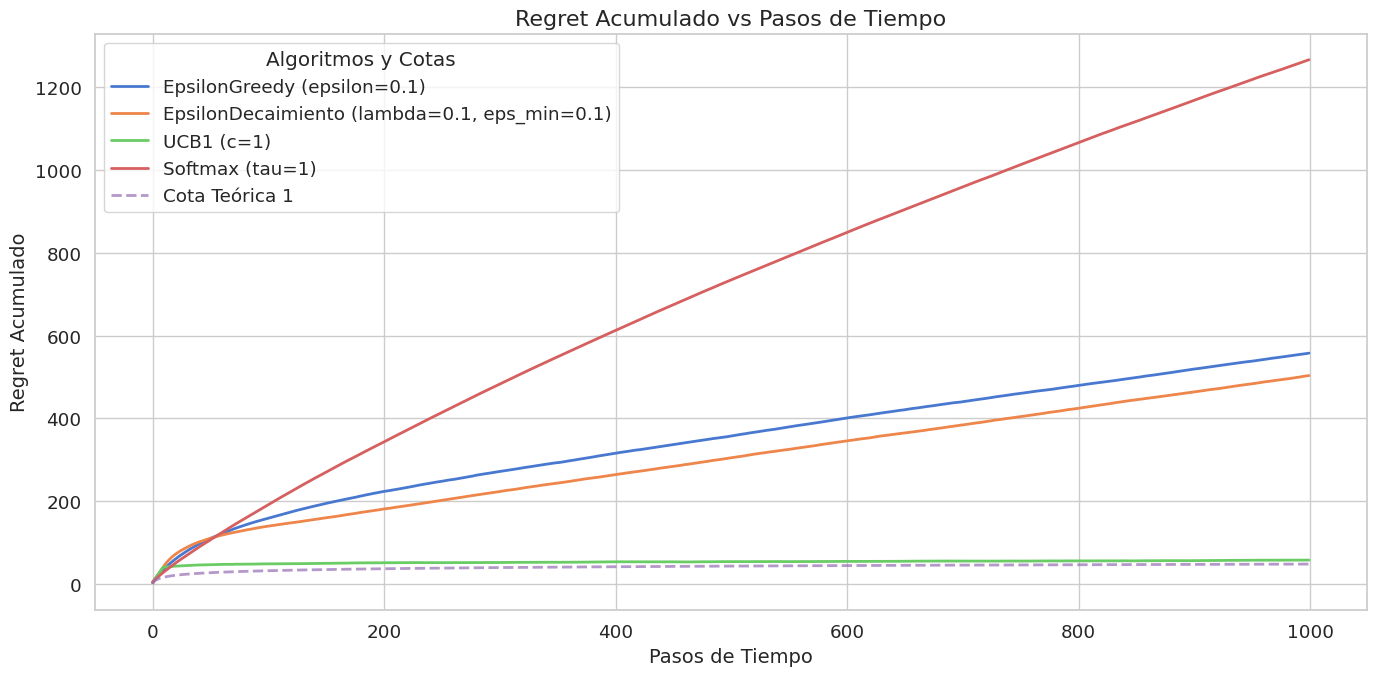
\includegraphics[width=\linewidth]{imagenes/Normal-regret-general-mejores-parametros.png}
    \caption{Regret acumulado en distribución normal para la mejor configuración
    de cada algoritmo. UCB1 ($c{=}1$) se aproxima a la cota teórica; el resto
    exhiben regret lineal o sublineal pero alejado del óptimo.}
    \label{fig:normal_general}
\end{figure}

\subsubsection*{Distribución binomial}

La distribución binomial ($B(10,p_i)$, $k{=}10$, $T{=}1000$, UCB1 con $T{=}500$) reproduce el patrón anterior con UCB1 dominante, pero la cota teórica es mayor (${\approx}90$) porque la KL entre binomiales es menor que entre normales para el mismo $\Delta$, lo que requiere más muestras para descartar brazos subóptimos. Softmax ($\tau{=}1$) vuelve a ser el peor, las recompensas enteras en $\{0,\ldots,10\}$ generan selección casi uniforme para esa temperatura. $\varepsilon$-Decaimiento mejora levemente a $\varepsilon$-Greedy gracias a la reducción progresiva de exploración, pero ambos exhiben regret lineal lejos del óptimo logarítmico.

\begin{table}[h]
    \centering
    \small
    \begin{tabular}{lcc}
        \toprule
        Algoritmo & Mejor config. & Regret \\
        \midrule
        $\varepsilon$-Greedy      & $\varepsilon{=}0{.}1$   & 550 \\
        $\varepsilon$-Decaimiento & $\lambda{=}0{.}1$       & 480 \\
        UCB1                      & $c{=}1$                 & \textbf{60}$^\dagger$ \\
        Softmax                   & $\tau{=}1$              & 1000 \\
        \midrule
        Cota teórica              & ---                     & ${\approx}90$ \\
        \bottomrule
    \end{tabular}
    \caption{Mejor configuración de cada algoritmo en distribución binomial.
    $^\dagger$Medido a $T{=}500$. En negrita, el mejor resultado.}
    \label{tab:binomial_best}
\end{table}

\begin{figure}[h]
    \centering
    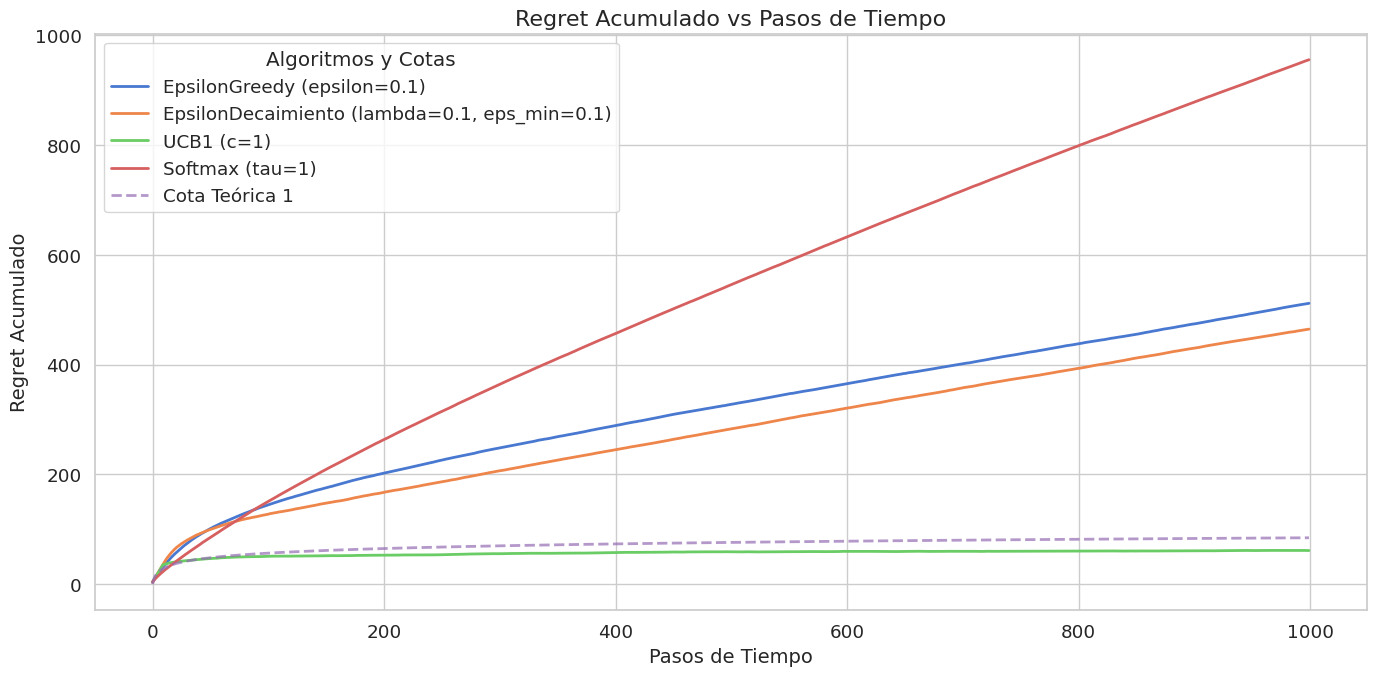
\includegraphics[width=\linewidth]{imagenes/Binomial-regret-general-mejores-parametros.png}
    \caption{Regret acumulado en distribución binomial para la mejor configuración
    de cada algoritmo.}
    \label{fig:binomial_general}
\end{figure}

\subsubsection*{Distribución Bernoulli}

La distribución Bernoulli ($\text{Bern}(p_i)$, $k{=}10$, $T{=}1000$, UCB1 con $T{=}500$) introduce un cambio cualitativo respecto a Normal y Binomial, al estar las recompensas en $\{0,1\}$, los algoritmos necesitan bonos de exploración y temperaturas más pequeñas. UCB1 con $c{=}0{.}1$ logra el mejor resultado (${\approx}25$), muy por debajo de la cota teórica (${\approx}75$), mientras que Softmax invierte su ranking habitual, ahora $\tau{=}0{.}1$ es el mejor (${\approx}100$) porque concentra eficazmente las selecciones en el brazo con mayor $\hat{p}$ estimada. $\varepsilon$-Greedy y $\varepsilon$-Decaimiento se aproximan a la cota teórica con sus mejores configuraciones.

\begin{table}[h]
    \centering
    \small
    \begin{tabular}{lcc}
        \toprule
        Algoritmo & Mejor config. & Regret \\
        \midrule
        $\varepsilon$-Greedy      & $\varepsilon{=}0{.}1$   & 70 \\
        $\varepsilon$-Decaimiento & $\lambda{=}0{.}1$       & 67 \\
        UCB1                      & $c{=}0{.}1$             & \textbf{25}$^\dagger$ \\
        Softmax                   & $\tau{=}0{.}1$          & 100 \\
        \midrule
        Cota teórica              & ---                     & ${\approx}85$ \\
        \bottomrule
    \end{tabular}
    \caption{Mejor configuración de cada algoritmo en distribución Bernoulli.
    $^\dagger$Medido a $T{=}500$. En negrita, el mejor resultado.}
    \label{tab:bernoulli_best}
\end{table}

\begin{figure}[h]
    \centering
    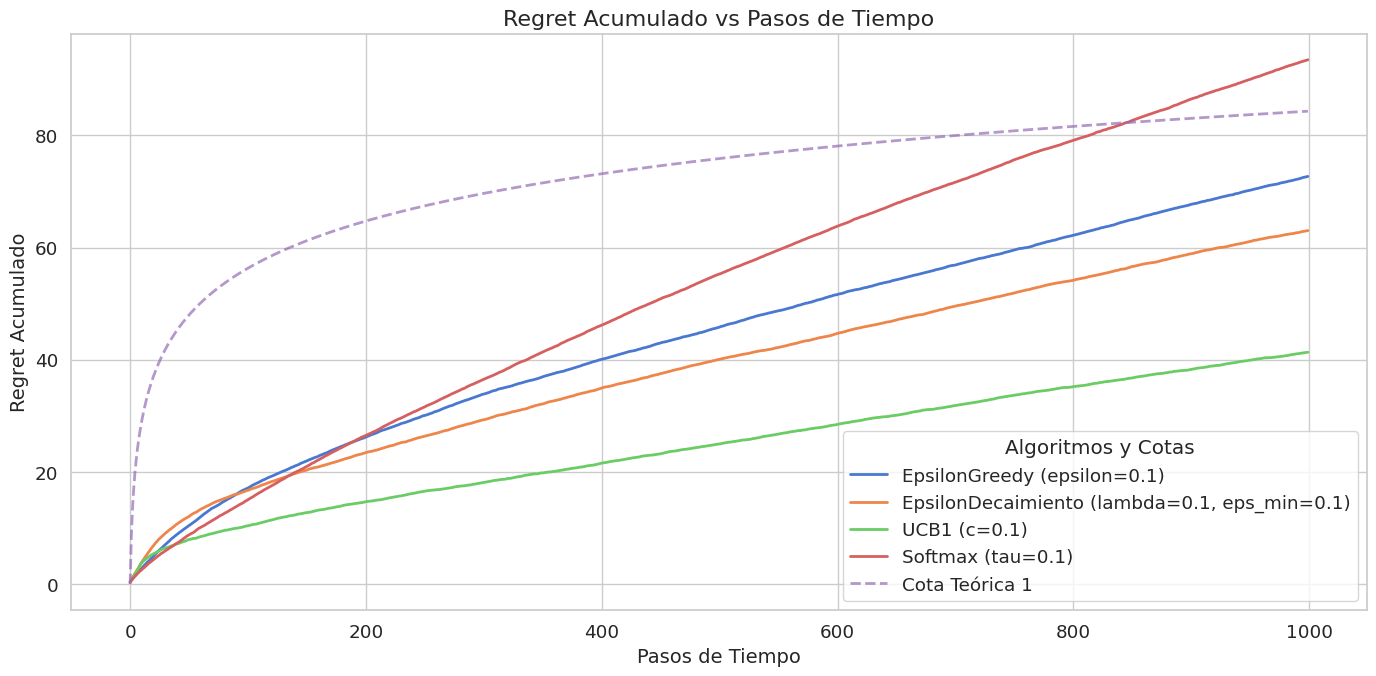
\includegraphics[width=\linewidth]{imagenes/Bernoulli-regret-general-mejores-parametros.png}
    \caption{Regret acumulado en distribución Bernoulli para la mejor configuración
    de cada algoritmo.}
    \label{fig:bernoulli_general}
\end{figure}


%%%%%%%%%%%%%%%%%%%%%%%%%%%%%%%%%%%%%%%%%%%%%%%%%%%%%%%%%%%%%
%%%%%%%%%%%%%%%%%%%%%%%%%%%%%%%%%%%%%%%%%%%%%%%%%%%%%%%%%%%%%   
\section{Conclusiones}
    %\begin{itemize}
    %    \item Un resumen de los principales resultados obtenidos.
    %    \item Limitaciones del estudio y posibles mejoras futuras.
    %    \item Reflexión sobre la importancia del trabajo y su impacto en el campo del aprendizaje por refuerzo.
    %    \item Líneas \textit{futuras} de estudio.
    %\end{itemize}

\textbf{UCB1 es el algoritmo más eficaz en las tres distribuciones estudiadas.} Es el único que logra regret sublineal próximo a la cota de Lai-Robbins, gracias a que su bono de confianza $c\sqrt{\ln t / N_i}$ equilibra exploración y explotación de forma adaptativa. Su parámetro óptimo depende de la escala de recompensas, $c{=}1$ para Normal y Binomial, $c{=}0{.}1$ para Bernoulli, donde las recompensas en $\{0,1\}$ requieren bonos más pequeños.

\textbf{La inicialización optimista transforma $\varepsilon$-Greedy.} Sin inicialización, el ranking es $\varepsilon{=}0{.}1 \succ \varepsilon{=}0{.}01 \succ \varepsilon{=}0$. con inicialización, se invierte: $\varepsilon{=}0$ y $\varepsilon{=}0{.}01$ pasan a ser los mejores (${\approx}145$) porque la fase de arranque forzado ya cubre la exploración necesaria. Es una heurística eficaz pero frágil, ya que requiere conocer la escala de recompensas de antemano.

\textbf{Softmax es el algoritmo más sensible a la distribución.} Su temperatura óptima es $\tau{=}1$ en Normal y Binomial, pero $\tau{=}0{.}1$ en Bernoulli. Un valor inadecuado produce exploración casi uniforme (regret lineal elevado), lo que lo convierte en el más difícil de ajustar en la práctica.

\textbf{La gráfica más relevante es el regret acumulado con cota teórica} (\texttt{plot\_regret}). Es la única que permite:
\begin{itemize}
    \item Cuantificar el coste de oportunidad real de cada algoritmo a lo largo del tiempo.
    \item Comparar directamente con la cota asintótica de Lai-Robbins, determinando si el algoritmo es óptimo en orden de magnitud.
    \item Distinguir regret sublineal ($O(\ln T)$) de lineal ($O(T)$), diferencia cualitativa invisible en \texttt{plot\_average\_rewards}.
\end{itemize}

\texttt{plot\_optimal\_selections} es complementaria, confirmando si la convergencia al brazo óptimo es consistente o puntual. \texttt{plot\_arm\_statistics} resulta útil para diagnóstico (detectar brazos ignorados) pero no para comparar algoritmos. \texttt{plot\_average\_rewards} aporta la menor información diferencial, al no referenciar el óptimo teórico.

\textbf{Limitaciones y líneas futuras.}
Los experimentos se limitan a $k{=}10$ y $T{\leq}1000$, con un único conjunto de brazos por distribución. Ampliar a horizontes mayores y múltiples instancias aleatorias (análisis de varianza del regret) daría resultados más robustos. Como extensión natural, Thompson Sampling y KL-UCB proporcionarían cotas más ajustadas para Bernoulli y Binomial, aprovechando la estructura discreta de sus distribuciones.


% MODIFICA EL CONTENIDO QUE VIENE A CONTINUACIÓN DE ACUERDO A TU TRABAJO

\chapter{Aprendizaje en Entornos Complejos}

%%%%%%%%%%%%%%%%%%%%%%%%%%%%%%%%%%%%%%%%%%%%%%%%%%%%%%%%%%%%%
%%%%%%%%%%%%%%%%%%%%%%%%%%%%%%%%%%%%%%%%%%%%%%%%%%%%%%%%%%%%%
\section{Introducción}

El aprendizaje por refuerzo representa una de las ramas más diversas de la inteligencia artificial, empleada para derrotar a campeones del mundo en juegos de mesa estratégicos o en la construcción de modelos de lenguaje avanzados. 
A diferencia del problema del bandido de $k$-brazos, donde las decisiones se toman en un entorno estático, los problemas del mundo real se desarrollan en un contexto dinámico. Cada decisión tomada por el agente modifica el estado del entorno, lo que requiere cálculos constantes para actualizar su percepción del mundo.

La motivación de este trabajo radica en comprender y aplicar algoritmos capaces de resolver tareas sin un conocimiento previo de la dinámica del entorno. Se pretende evolucionar desde los métodos tabulares clásicos, viables en espacios de estados reducidos, hasta el control con aproximaciones de función mediante redes neuronales, necesario para abordar entornos continuos y complejos.

Los objetivos principales de este informe son:
\begin{enumerate}
    \item Implementar y comparar el rendimiento de algoritmos de control tabular (Monte Carlo, SARSA y Q-Learning) en entornos de estados discretos.
    \item Desarrollar y evaluar algoritmos de control aproximado (Deep Q-Learning y SARSA semi-gradiente) en entornos continuos.
    \item Analizar el comportamiento, el rendimiento y la convergencia de los agentes basándose en la librería de gymnasium \cite{gymnasium} para llevar a cabo las pruebas.
\end{enumerate}

El documento se organiza de la siguiente manera: la sección de Desarrollo detalla el marco teórico necesario para aplicar los algoritmos de aprendizaje. La sección de Algoritmos expone el pseudocódigo y la lógica de los métodos implementados. Posteriormente, la Evaluación presenta los resultados empíricos obtenidos en los entornos seleccionados, y finalmente, se extraen las Conclusiones y líneas de mejora futuras.

%%%%%%%%%%%%%%%%%%%%%%%%%%%%%%%%%%%%%%%%%%%%%%%%%%%%%%%%%%%%%
%%%%%%%%%%%%%%%%%%%%%%%%%%%%%%%%%%%%%%%%%%%%%%%%%%%%%%%%%%%%%
\section{Desarrollo}

\subsection{Definición Formal del Problema}

El aprendizaje en entornos complejos se formaliza a través de un Proceso de Decisión de Markov (MDP). Un MDP se define mediante la tupla $\langle \mathcal{S}, \mathcal{A}, \mathcal{\{{P^a}\}_a}, \mathcal{R}, \gamma \rangle$, donde en cada instante $t$, el agente observa un estado $S_t \in \mathcal{S}$, ejecuta una acción $A_t \in \mathcal{A}$ siguiendo una política $\pi(a|s)$, y transita a un nuevo estado $S_{t+1}$ recibiendo una recompensa $R_{t+1}$.

\begin{definition}[Política]
Una política, representada como $\pi$, es una función que indica qué acción realizar de acuerdo al estado actual del entorno. Puede ser determinista, asignando una acción fija a un estado, o estocástica, proporcionando una distribución de probabilidad sobre las acciones posibles.
\end{definition}

El objetivo del agente es encontrar la política óptima $\pi^*$ que maximice el retorno esperado (la suma de recompensas descontadas a futuro):
\begin{equation}
    G_t = \sum_{k=0}^{\infty} \gamma^k R_{t+k+1}
\end{equation}

Para poder escoger la acción que lleve a un estado donde la recompensa sea máxima, el agente construye una representación interna del entorno basado en sus experiencias anteriores. La puntuación que asigna a cada estado el agente se basa en las ecuaciones de Bellman, que según el algoritmo implementado, se modifica para poder aplicar distintos enfoques. La fórmula general es la siguiente

\begin{equation}
    v(s) = \mathbb{E}[R_{t+1} + \gamma v(S_{t+1}) \mid S_t = s]
\end{equation}

Esta fórmula desglosa el valor de un estado en dos componentes principales:
\begin{itemize}
    \item \textbf{$R_{t+1}$:} Es la recompensa inmediata que el agente recibe al realizar una transición desde el estado actual $s$.
    \item \textbf{$\gamma v(S_{t+1})$:} Representa el valor del siguiente estado ($S_{t+1}$) multiplicado por el factor de descuento $\gamma$. Este factor determina la importancia de las recompensas futuras frente a las inmediatas.
\end{itemize}

Esta ecuación representa que el valor de un estado es la recompensa inmediata más un valor a futuro, que representa el pasar a un próximo estado.

Para aplicar esta ecuación a cierto problema, se necesitan datos que involucren la obtención de recompensas.
\begin{definition}[Episodio]
Un episodio se define como una secuencia que involucra pasar por un estado, tomar una acción y obtener una recompensa por alcanzar otro estado, terminando el episodio en un estado terminal teoricamente. En tareas episódicas, el agente utiliza la retroalimentación obtenida al final o durante el transcurso del episodio para maximizar la recompensa acumulativa futura
\end{definition}

\subsection{Enfoques y Métodos Utilizados}

Cuando no se conoce el modelo de transiciones $\mathcal{P}$ ni la función de recompensa $\mathcal{R}$, el agente debe aprender a través de la experiencia. El objetivo que tiene este es actualizar su representación del entorno (tabla de estados-acciones $Q$) para poder elegir, dado un estado $S$, la acción $A$ que maximice su retorno. Las familias de métodos estudiadas se muestran a continuación por antigüedad.

\begin{itemize}
    \item \textbf{Métodos de Monte Carlo (MC):} Requieren que el episodio termine para calcular el retorno real $G_t$ y actualizar el valor de los estados visitados. Son métodos de alta varianza pero sin sesgo.
    \item \textbf{Métodos de Diferencias Temporales (TD):} Combinan ideas de MC y Programación Dinámica. Actualizan las estimaciones basándose en otras estimaciones parciales (bootstrapping) paso a paso, sin esperar al final del episodio.
    \item \textbf{Control con Aproximaciones:} Cuando el espacio de estados es inmenso o continuo, es imposible mantener una tabla $Q(s,a)$. Se opta por aproximar la función de valor como una forma funcional parametrizada con un vector de pesos.
\end{itemize}

Estos enfoques mejoran gradualmente la aplicabilidad del agente. Los métodos TD mejoran a MC en entornos largos o continuos al aprender paso a paso, mientras que los métodos aproximados (DQN) suponen el salto cualitativo definitivo para resolver tareas complejas inabarcables mediante técnicas tabulares. 

Aunque los últimos métodos mencionados sean los más complejos, en \cite{qlearningtrafico} se utilizó Q-Learning con ciertas optimizaciones para la optimización del movimiento de aeronaves en tierra dentro de los aeropuertos, demostrando ser más eficiente que los métodos tradicionales. Otro ejemplo conocido que usaba métodos aproximados es el de \cite{atariDQN}, donde se usó Deep Q-Learning para conseguir resultados propios del estado del arte en cuanto a rendimiento en juegos de la consola Atari 2600, introduciendo únicamente píxeles como input a la red.

Este trabajo se diferencia de otros enfoques previos al alejarse de la mera réplica de tutoriales para establecer y seguir un criterio de evaluación y una metodología propia.

%%%%%%%%%%%%%%%%%%%%%%%%%%%%%%%%%%%%%%%%%%%%%%%%%%%%%%%%%%%%%
%%%%%%%%%%%%%%%%%%%%%%%%%%%%%%%%%%%%%%%%%%%%%%%%%%%%%%%%%%%%%
\section{Algoritmos}

A continuación, se describen los algoritmos estudiados. Todos los agentes siguen la misma interfaz estructural basada en los métodos \texttt{get\_action(obs)} y \texttt{update(...)} típica de gymnasium.

\subsection*{Monte Carlo Control (Off-policy)}
Este algoritmo separa la política que se está aprendiendo (objetivo, $\pi$) de la política que genera el comportamiento (comportamiento o behavior, $b$), permitiendo aprender una política determinista óptima a partir de datos generados por una política exploratoria $\varepsilon$-soft. La diferencia entre las dos políticas se corrige mediante muestreo por importancia ponderado.

\begin{algorithm}
\caption{Control de Monte Carlo (off-policy)}\label{algo:mc_off_policy}
\begin{algorithmic}[1]
\State \textbf{Inicializar, para todo $s \in \mathcal{S}, a \in \mathcal{A}(s)$:}
    \State $Q(s, a) \in \mathbb{R}$ (arbitrariamente)
    \State $C(s, a) \gets 0$
    \State $\pi(s) \gets \arg\max_a Q(s, a)$ \Comment{con empates rotos consistentemente}
\State \textbf{Repetir para siempre (para cada episodio):}
    \State $b \gets$ cualquier política blanda (\textit{soft policy})
    \State Generar un episodio usando $b$: $S_0, A_0, R_1, \dots, S_{T-1}, A_{T-1}, R_T$
    \State $G \gets 0$
    \State $W \gets 1$
    \For{$t = T-1, T-2, \dots, 0$}
        \State $G \gets \gamma G + R_{t+1}$
        \State $C(S_t, A_t) \gets C(S_t, A_t) + W$
        \State $Q(S_t, A_t) \gets Q(S_t, A_t) + \dfrac{W}{C(S_t, A_t)} \bigl[ G - Q(S_t, A_t) \bigr]$
        \State $\pi(S_t) \gets \arg\max_a Q(S_t, a)$ \Comment{con empates rotos consistentemente}
        \If{$A_t \neq \pi(S_t)$} 
            \State \textbf{salir del bucle interno} \Comment{proceder al siguiente episodio}
        \EndIf
        \State $W \gets W \dfrac{1}{b(A_t|S_t)}$
    \EndFor
\end{algorithmic}
\end{algorithm}

A pesar de que en la práctica los algoritmos de diferencias temporales suelen ser más eficientes, el concepto de Monte Carlo se aplica en algoritmos más complejos como REINFORCE que se basa en el gradiente de política.

\subsection*{Monte Carlo Control First-Visit (On-policy)}
Este algoritmo es un caso concreto del anterior, donde la política de comportamiento y la política objetivo son la misma. Además solo se actualiza un par (estado,valor) la primera vez que aparece en un episodio.

\subsection*{Sarsa (on-policy TD control)}
A diferencia de los métodos de Monte Carlo, Sarsa es un algoritmo de Diferencias Temporales (TD) que actualiza la tabla de valores $Q$ cada paso (con TD(0)). Es un método on-policy ya que utiliza la misma política para obtener la próxima acción del agente, necesaria para calcular el valor esperado del estado actual.

\begin{algorithm}[h]
\caption{Sarsa: Control TD en la política (on-policy) para estimar $Q \approx q_*$}\label{algo:sarsa}
\begin{algorithmic}[1]
\Require Parámetros del algoritmo: tamaño de paso $\alpha \in (0, 1]$, $\varepsilon > 0$ pequeño
\State Inicializar $Q(s, a)$, para todo $s \in \mathcal{S}^+, a \in \mathcal{A}(s)$, arbitrariamente excepto que $Q(terminal, \cdot) = 0$
\For{cada episodio}
    \State Inicializar $S$
    \State Elegir $A$ desde $S$ usando una política derivada de $Q$ (p.e., $\varepsilon$-greedy)
    \While{$S$ no sea terminal}
        \State Realizar la acción $A$, observar $R$ y el siguiente estado $S'$
        \State Elegir $A'$ desde $S'$ usando una política derivada de $Q$ (p.e., $\varepsilon$-greedy)
        \State $Q(S, A) \gets Q(S, A) + \alpha \bigl[ R + \gamma Q(S', A') - Q(S, A) \bigr]$
        \State $S \gets S'$
        \State $A \gets A'$
    \EndWhile
\EndFor
\end{algorithmic}
\end{algorithm}
SARSA es un algoritmo que toma en cuenta sus decisiones en el futuro, por lo que su política se vuelve más conservadora.

\subsection*{Q-Learning (off-policy TD control)}
Este es un método off-policy que actualiza $Q(S, A)$ asumiendo que en el siguiente estado se tomará la acción óptima ($\max_a Q(S', a)$), incluso si el agente termina realizando una acción diferente por exploración.
\begin{algorithm}[!h]
\caption{Q-learning: Control TD fuera de la política (off-policy) para estimar $\pi \approx \pi_*$}\label{algo:q_learning_tabular}
\begin{algorithmic}[1]
\Require Parámetros del algoritmo: tamaño de paso $\alpha \in (0, 1]$, $\varepsilon > 0$ pequeño
\State Inicializar $Q(s, a)$, para todo $s \in \mathcal{S}^+, a \in \mathcal{A}(s)$, arbitrariamente excepto que $Q(terminal, \cdot) = 0$
\For{cada episodio}
    \State Inicializar $S$
    \Repeat \Comment{Para cada paso del episodio}
        \State Elegir $A$ desde $S$ usando una política derivada de $Q$ (p.e., $\varepsilon$-greedy)
        \State Realizar la acción $A$, observar $R$ y el siguiente estado $S'$
        \State $Q(S, A) \gets Q(S, A) + \alpha \bigl[ R + \gamma \max_a Q(S', a) - Q(S, A) \bigr]$
        \State $S \gets S'$
    \Until{$S$ es terminal}
\EndFor
\end{algorithmic}
\end{algorithm}
Q-Learning, al ser off-policy, se aproxima más a la política óptima que SARSA debido a que su política objetivo es greedy y siempre escoge el estado con máximo valor.

\subsection*{Sarsa semi-gradiente episódico}
A diferencia de los métodos tabulares, SARSA semi-gradiente utiliza una función de valor de acción parametrizada ($\hat{q}$) y actualiza un vector de pesos ($\mathbf{w}$) mediante descenso de gradiente para generalizar el aprendizaje en espacios de estados grandes o continuos.
\begin{algorithm}[!h]
\caption{Sarsa semi-gradiente episódico para estimar $\hat{q} \approx q_*$}\label{algo:semi_gradient_sarsa}
\begin{algorithmic}[1]
\State \textbf{Entrada:} una parametrización de función de valor de acción diferenciable $\hat{q} : \mathcal{S} \times \mathcal{A} \times \mathbb{R}^d \to \mathbb{R}$
\Require tamaño de paso $\alpha > 0$, $\varepsilon > 0$ pequeño
\State Inicializar los pesos de la función de valor $\mathbf{w} \in \mathbb{R}^d$ arbitrariamente (p.e., $\mathbf{w} = \mathbf{0}$)
\For{cada episodio}
    \State $S, A \gets$ estado y acción inicial del episodio (p.e., $\varepsilon$-greedy)
    \While{$S$ no sea terminal}
        \State Realizar la acción $A$, observar $R$ y el siguiente estado $S'$
        \If{$S'$ es terminal}
            \State $\mathbf{w} \gets \mathbf{w} + \alpha \bigl[ R - \hat{q}(S, A, \mathbf{w}) \bigr] \nabla \hat{q}(S, A, \mathbf{w})$
            \State \textbf{ir al siguiente episodio}
        \EndIf
        \State Elegir $A'$ como una función de $\hat{q}(S', \cdot, \mathbf{w})$ (p.e., $\varepsilon$-greedy)
        \State $\mathbf{w} \gets \mathbf{w} + \alpha \bigl[ R + \gamma \hat{q}(S', A', \mathbf{w}) - \hat{q}(S, A, \mathbf{w}) \bigr] \nabla \hat{q}(S, A, \mathbf{w})$
        \State $S \gets S'$
        \State $A \gets A'$
    \EndWhile
\EndFor
\end{algorithmic}
\end{algorithm}

Este algoritmo permite manejar espacios de estado enormes o continuos al no depender de una tabla de valores $Q$.

\subsection*{Deep Q-Learning (DQN) con Experience Replay}
DQN extiende Q-Learning aproximando $q(s,a)$ con una red neuronal profunda $\hat{q}(s,a;\mathbf{w})$ que recibe el estado como entrada y devuelve los valores de todas las acciones posibles. Para estabilizar el aprendizaje utiliza \textit{Experience Replay} (muestreo aleatorio de transiciones almacenadas) y una \textit{Target Network} con parámetros congelados $\mathbf{w}^-$ que reduce la oscilación del target.

\begin{algorithm}[!h]
\caption{Deep Q-Learning con Experience Replay}\label{algo:dqn}
\begin{algorithmic}[1]
\State Inicializar memoria de repetición $D$ con capacidad $N$
\State Inicializar red $Q$ con pesos aleatorios $\mathbf{w}$
\State Inicializar red objetivo con $\mathbf{w}^- \gets \mathbf{w}$
\For{cada episodio}
    \State Inicializar estado $s_1$
    \For{$t=1$ hasta $T$}
        \State Con probabilidad $\epsilon$ elegir acción aleatoria; si no, $a_t=\arg\max_a \hat{q}(s_t,a;\mathbf{w})$
        \State Ejecutar $a_t$, observar $r_t$, $s_{t+1}$ y $done$
        \State Guardar $(s_t,a_t,r_t,s_{t+1},done)$ en $D$
        \State Muestrear un minibatch aleatorio de $D$
        \For{cada transición $(s_j,a_j,r_j,s_{j+1},done_j)$}
            \If{$done_j$}
                \State $y_j \gets r_j$
            \Else
                \State $y_j \gets r_j + \gamma \max_{a'} \hat{q}(s_{j+1},a';\mathbf{w}^-)$
            \EndIf
        \EndFor
        \State Actualizar $\mathbf{w}$ con un paso de gradiente sobre $(y_j-\hat{q}(s_j,a_j;\mathbf{w}))^2$
        \State Cada $C$ pasos: $\mathbf{w}^- \gets \mathbf{w}$
    \EndFor
\EndFor
\end{algorithmic}
\end{algorithm}

DQN es off-policy y permite escalar Q-Learning a espacios de estados continuos o de alta dimensión, manteniendo el control mediante una política $\epsilon$-greedy sobre la red.
%%%%%%%%%%%%%%%%%%%%%%%%%%%%%%%%%%%%%%%%%%%%%%%%%%%%%%%%%%%%%
%%%%%%%%%%%%%%%%%%%%%%%%%%%%%%%%%%%%%%%%%%%%%%%%%%%%%%%%%%%%%
\section{Evaluación/Experimentos}

\subsection{Configuración Experimental}

Las pruebas se realizaron con la librería Gymnasium y semilla fija (SEED=2024) para garantizar reproducibilidad. Se estudiaron tres entornos representativos:

\begin{itemize}
    \item \textbf{Taxi-v3 (discreto):} 500 estados, 6 acciones. Recompensas: $-1$ por paso, $+20$ entrega exitosa, $-10$ acción ilegal. Entrenamiento de 100\,000 episodios para comparar MC, SARSA y Q-Learning.
    \item \textbf{CliffWalking-v1 (discreto):} grid 4$\times$12 (48 estados), 4 acciones. Recompensas: $-1$ por paso, $-100$ caída al acantilado y $0$ al llegar. Entrenamiento de 10\,000 episodios para comparar Q-Learning vs SARSA.
    \item \textbf{LunarLander-v3 (continuo):} estado de 8 variables continuas y 4 acciones discretas: $0$ (no hacer nada), $1$ (motor lateral izquierdo), $2$ (motor principal), $3$ (motor lateral derecho). Elegimos el espacio de acciones discreto porque DQN y SARSA-SG están formulados para acciones discretas; usar el espacio continuo exigiría métodos de política/actor-crítico (p.ej., DDPG/PPO). Entrenamiento de 5\,000 episodios para DQN y SARSA semi-gradiente.
\end{itemize}

Parámetros base utilizados:

\begin{itemize}
    \item \textbf{Tabulares (Taxi):} $\epsilon$-greedy con decaimiento $\epsilon_t=\min(1,1000/(t+1))$, $\alpha=0.1$, $\gamma=1.0$.
    \item \textbf{Tabulares (Cliff):} $\epsilon$-greedy con el mismo decaimiento, $\alpha=0.1$, $\gamma=0.99$.
    \item \textbf{DQN (base):} $\alpha=0.0005$, $\gamma=0.99$, buffer 50k, batch 64, target update $C=2000$, red 64$\times$64, $\epsilon$ decay $0.999$ (mínimo 0.01).
    \item \textbf{SARSA-SG (base):} $\alpha=0.001$, $\gamma=0.99$, red 64$\times$64, $\epsilon$ decay $0.995$ (mínimo 0.01).
\end{itemize}

\subsection{Métricas}

Para evaluar el aprendizaje se midieron tres indicadores:
\begin{itemize}
    \item \textbf{Recompensa media acumulada por episodio}: $\bar{R}_t = \frac{1}{t}\sum_{i=1}^{t} R_i$. En entornos con fuertes penalizaciones iniciales (CliffWalking) esta métrica puede permanecer muy negativa.
    \item \textbf{Longitud media de episodios}: número de pasos por episodio (se reporta la media de los últimos 1000 episodios).
    \item \textbf{Pérdida (solo DQN)}: evolución de la loss Huber para analizar estabilidad del entrenamiento.
\end{itemize}

\subsection{Resultados y Análisis Crítico}

\subsubsection*{Taxi-v3 (control tabular)}
Como se aprecia en la Figura~\ref{fig:taxi-recompensa}, la comparación conjunta (misma configuración de hiperparámetros) confirma que los métodos TD superan claramente a Monte Carlo en velocidad de convergencia.

\begin{table}[h]
\centering
\resizebox{\columnwidth}{!}{%
\begin{tabular}{lcc}
\hline
\textbf{Algoritmo} & \textbf{Recompensa media final} & \textbf{Longitud media final (pasos)} \\
\hline
MC On-Policy & -138.82 & 113.73 \\
MC Off-Policy & -22.32 & 13.69 \\
SARSA & -5.34 & 13.04 \\
Q-Learning & -4.47 & 13.06 \\
\hline
\end{tabular}%
}
\caption{Resultados en Taxi-v3 (100k episodios).}
\end{table}

Los métodos TD convergen en pocos miles de episodios, mientras que MC on-policy queda anclado en episodios largos, como se ve en la Figura~\ref{fig:taxi-pasos}. Q-Learning y SARSA terminan prácticamente empatados en Taxi-v3 (recompensa -4.47 vs -5.34 y longitud 13.06 vs 13.04), lo que indica que en este entorno la diferencia on/off-policy apenas se nota; la dinámica no penaliza de forma fuerte la exploración. Por eso, para analizar con más claridad esa diferencia, se evalúa después CliffWalking, donde el riesgo de caer introduce un contraste real entre ambos métodos. En Q-Learning, un $\epsilon$ fijo muy bajo (0.01) da recompensas positivas (6.31), mientras que $\gamma=0.05$ no aprende (longitud media 82.97 pasos) porque el descuento es tan fuerte que la recompensa final no se propaga hacia atrás, tal como muestran las curvas de la Figura~\ref{fig:taxi-qlearn-hypers}. En SARSA ocurre algo similar: $\epsilon=0.01$ mejora el rendimiento (recompensa 6.26, 13.25 pasos) y $\gamma=0.25$ lo degrada claramente (recompensa -159.61, 112.51 pasos) al reducir demasiado la importancia del retorno futuro, visible en la Figura~\ref{fig:taxi-sarsa-hypers}.

\begin{figure}[!htbp]
    \centering
    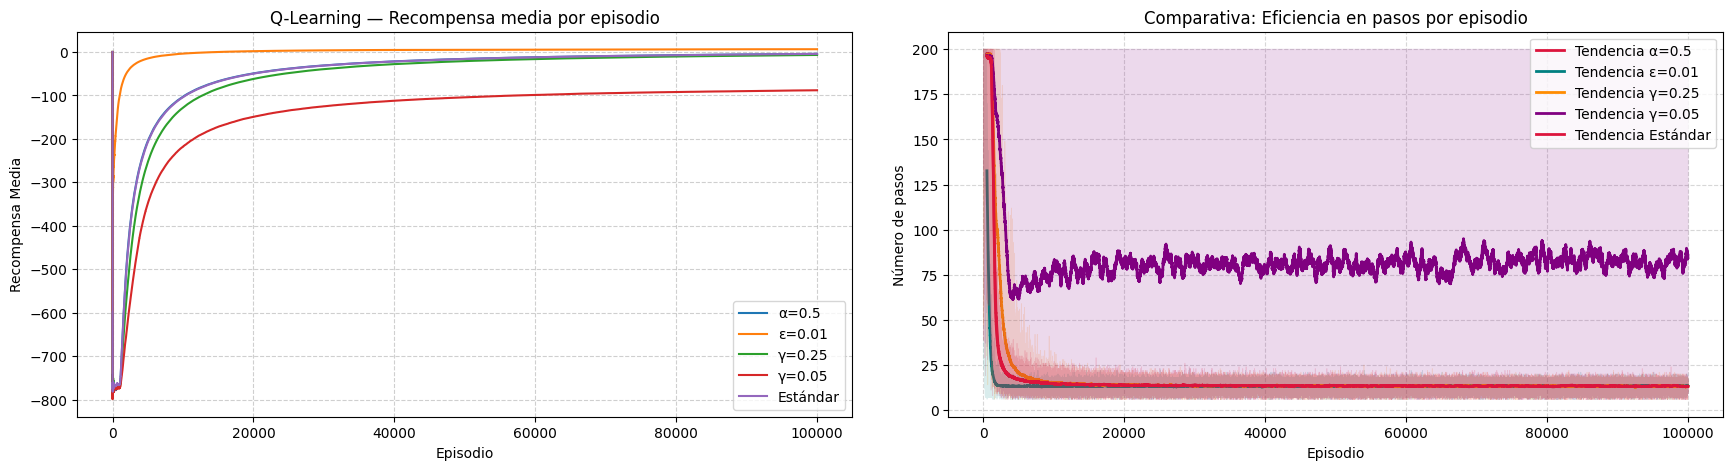
\includegraphics[width=0.95\linewidth]{imagenes/taxi_qlearning_hyper_combo.png}
    \caption{Taxi-v3: Q-Learning con variaciones de $\alpha$, $\epsilon$ y $\gamma$.}
    \label{fig:taxi-qlearn-hypers}
\end{figure}

\begin{figure}[!htbp]
    \centering
    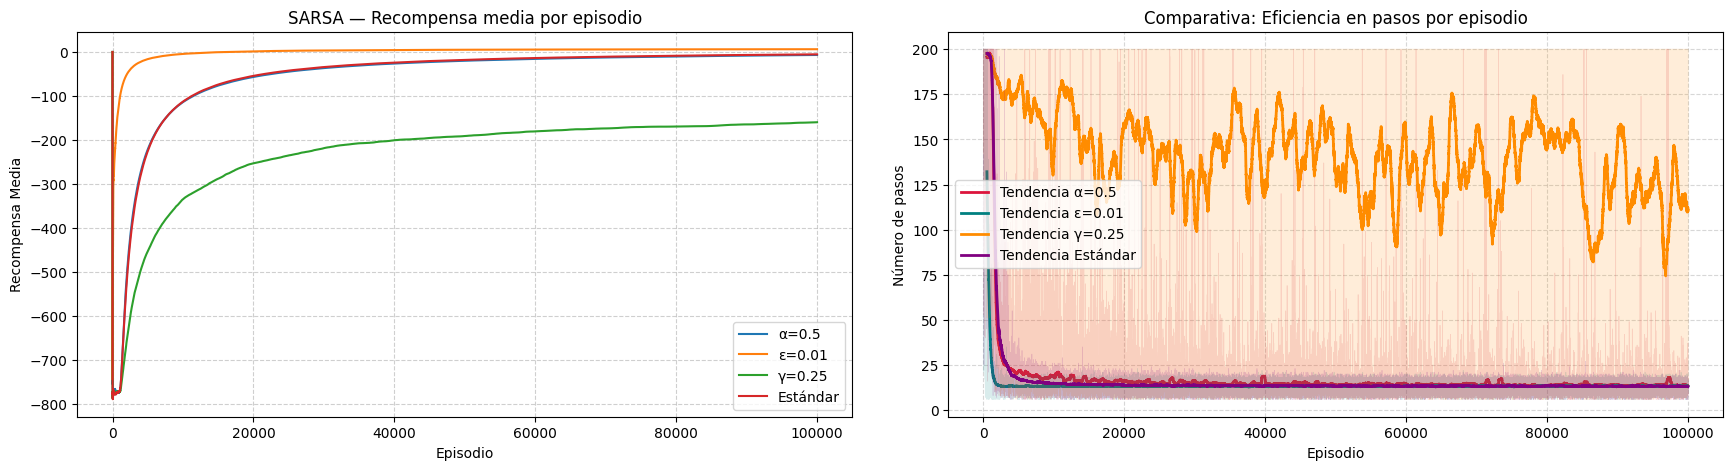
\includegraphics[width=0.95\linewidth]{imagenes/taxi_sarsa_hyper_combo.png}
    \caption{Taxi-v3: SARSA con variaciones de $\alpha$, $\epsilon$ y $\gamma$.}
    \label{fig:taxi-sarsa-hypers}
\end{figure}

La diferencia entre MC on-policy y off-policy es clara: con on-policy el agente mantiene mucha exploración y los episodios permanecen largos, mientras que off-policy puede seguir una política objetivo más greedy y reduce rápidamente la longitud. Esto se aprecia en la Figura~\ref{fig:taxi-pasos}, donde MC on-policy se estabiliza alrededor de 110–120 pasos, y MC off-policy cae a valores cercanos a 14–15 pasos, alineados con SARSA y Q-Learning.

\begin{figure}[!htbp]
    \centering
    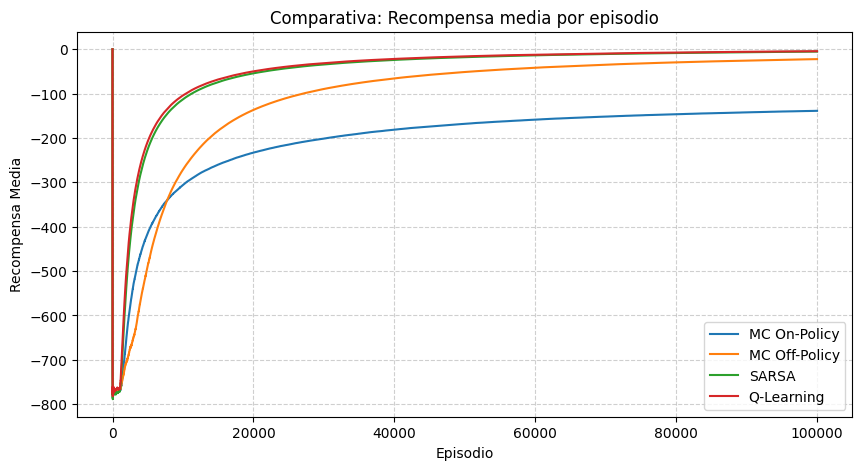
\includegraphics[width=0.9\linewidth]{imagenes/taxi_comparativa_recompensa.png}
    \caption{Taxi-v3: recompensa media por episodio (MC on/off, SARSA y Q-Learning).}
    \label{fig:taxi-recompensa}
\end{figure}

\begin{figure}[!htbp]
    \centering
    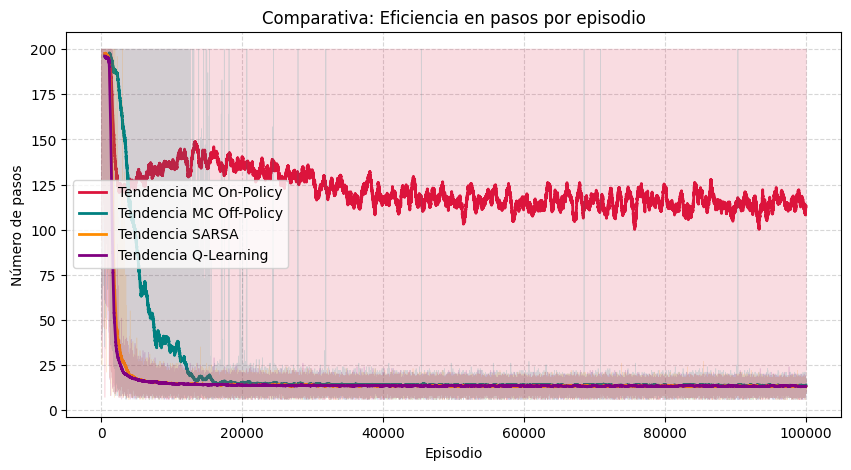
\includegraphics[width=0.9\linewidth]{imagenes/taxi_comparativa_pasos.png}
    \caption{Taxi-v3: eficiencia en pasos por episodio (tendencias suavizadas).}
    \label{fig:taxi-pasos}
\end{figure}

\subsubsection*{CliffWalking-v1 (riesgo vs optimalidad)}
Aquí se observa la diferencia on-policy/off-policy. Q-Learning converge a la ruta óptima (13 pasos) en el episodio greedy, mientras SARSA aprende la ruta segura (17 pasos) porque, al ser on-policy, internaliza el riesgo de sus propias acciones exploratorias. La media acumulada refleja muchas caídas iniciales porque al explorar el agente cae con frecuencia al acantilado y recibe una penalización fuerte (-100), lo que mantiene la media muy negativa durante los primeros miles de episodios (Figura~\ref{fig:cliff-recompensa}):

\begin{itemize}
    \item Q-Learning: recompensa media final -6845.23, longitud media 17.08 pasos.
    \item SARSA: recompensa media final -8025.64, longitud media 19.33 pasos.
\end{itemize}

Con $\epsilon=0.01$ ambos mejoran notablemente: Q-Learning se acerca a 13.36 pasos y SARSA a 15.19 pasos. En Q-Learning, $\gamma=0.05$ falla (longitud media $>180$ pasos). La eficiencia en pasos durante el entrenamiento se compara en la Figura~\ref{fig:cliff-pasos}.

\begin{figure}[!htbp]
    \centering
    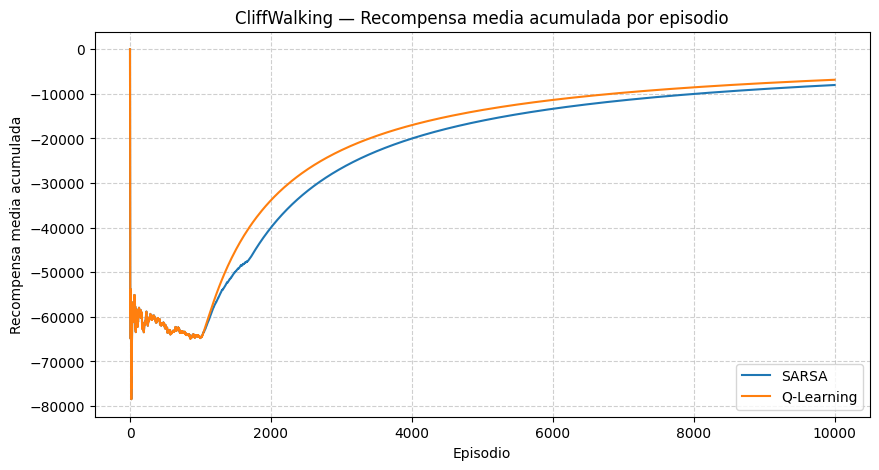
\includegraphics[width=0.9\linewidth]{imagenes/cliff_comparativa_recompensa.png}
    \caption{CliffWalking-v1: recompensa media acumulada por episodio (SARSA vs Q-Learning).}
    \label{fig:cliff-recompensa}
\end{figure}

\begin{figure}[!htbp]
    \centering
    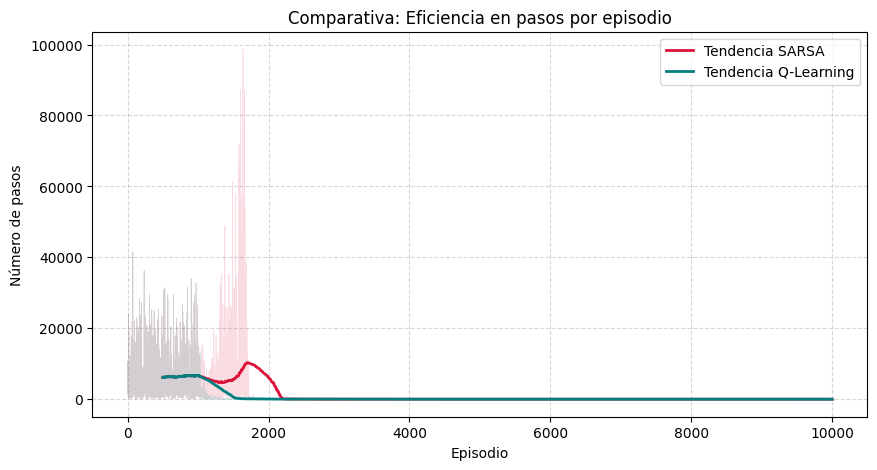
\includegraphics[width=0.9\linewidth]{imagenes/cliff_comparativa_pasos.png}
    \caption{CliffWalking-v1: eficiencia en pasos por episodio (SARSA vs Q-Learning).}
    \label{fig:cliff-pasos}
\end{figure}

\subsubsection*{LunarLander-v3 (control aproximado)}
En el entorno continuo se requiere aproximación de función. Con los hiperparámetros base, SARSA-SG alcanza recompensa superior pero DQN obtiene episodios más cortos:

\begin{itemize}
    \item SARSA-SG (base 64x64): recompensa media final 176.38, longitud media 295.29 pasos.
    \item DQN (base): recompensa media final 118.11, longitud media 206.23 pasos.
\end{itemize}

La sensibilidad de DQN a sus hiperparámetros es clara: con $C=50$ la recompensa cae a -493.42, mientras que $C=10000$ mejora ligeramente (129.99), como se ve en la Figura~\ref{fig:lunar-dqn-target}. En el barrido del buffer (Figura~\ref{fig:lunar-dqn-buffer}), la configuración base (50k) ronda 118 puntos, pero al reducirlo a 5k baja a 51.47 y con 1k se desploma a 18.60, evidenciando la necesidad de decorrelación temporal.

En SARSA-SG, el barrido de arquitectura también muestra diferencias: una red 128$\times$128 alcanza 173.93 con 265.23 pasos, mientras que una 16$\times$16 cae a 106.02 y 417.75 pasos, confirmando que la capacidad de la función aproximadora es crítica en LunarLander (Figura~\ref{fig:lunar-sarsa-arch}). La comparación directa entre ambos métodos se muestra en las Figuras~\ref{fig:lunar-comp-recompensa} y~\ref{fig:lunar-comp-pasos}.

\begin{figure}[!htbp]
    \centering
    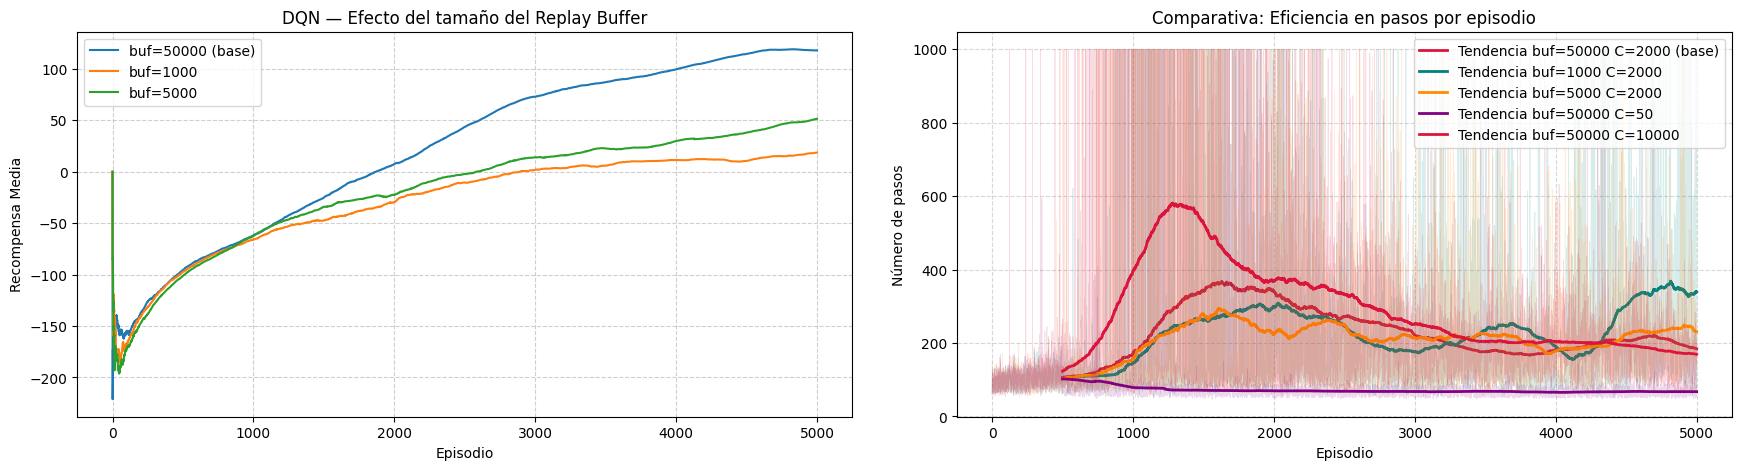
\includegraphics[width=0.95\linewidth]{imagenes/lunar_dqn_buffer_combo.png}
    \caption{LunarLander-v3: DQN — efecto del tamaño del Replay Buffer.}
    \label{fig:lunar-dqn-buffer}
\end{figure}

\begin{figure}[!htbp]
    \centering
    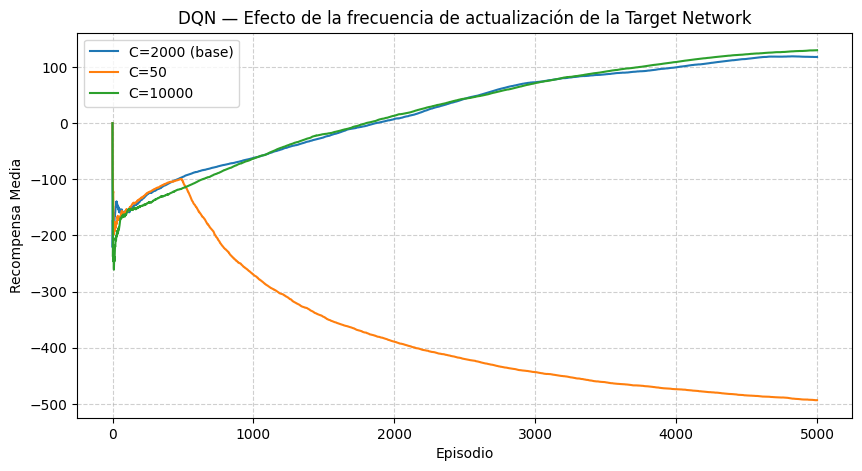
\includegraphics[width=0.9\linewidth]{imagenes/lunar_dqn_target_recompensa.png}
    \caption{LunarLander-v3: DQN — efecto de la frecuencia de actualización de la Target Network ($C$).}
    \label{fig:lunar-dqn-target}
\end{figure}

\begin{figure}[!htbp]
    \centering
    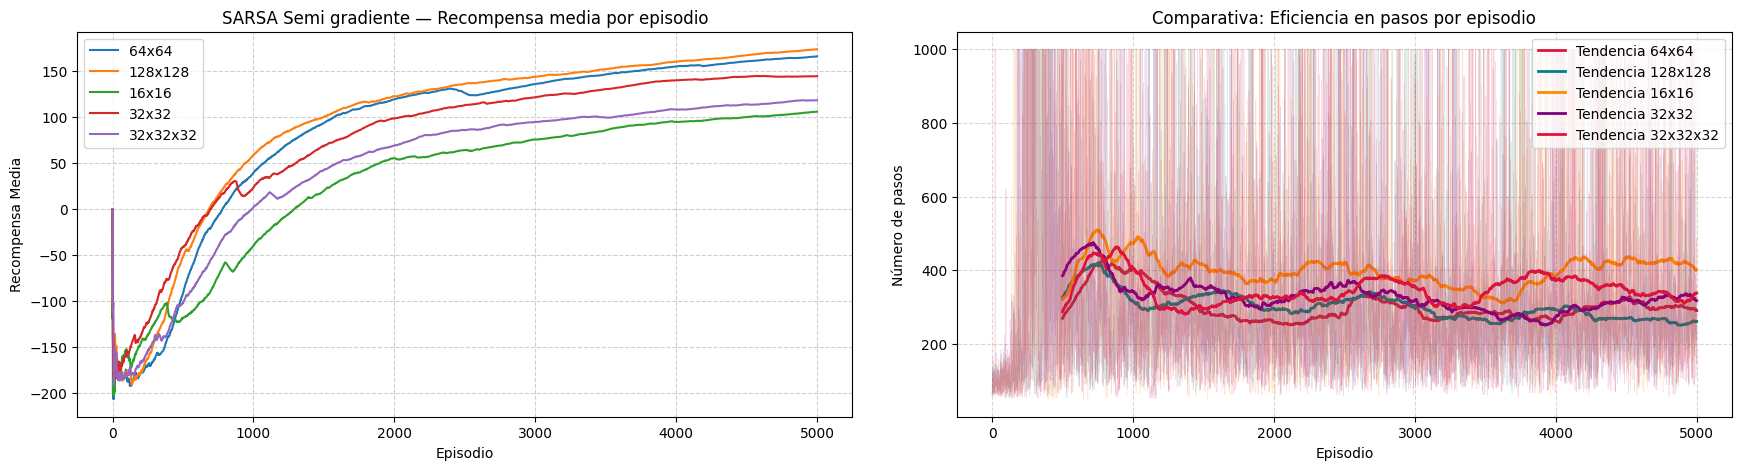
\includegraphics[width=0.95\linewidth]{imagenes/lunar_sarsa_sg_arch_combo.png}
    \caption{LunarLander-v3: SARSA-SG — efecto de la arquitectura de red.}
    \label{fig:lunar-sarsa-arch}
\end{figure}

\begin{figure}[!htbp]
    \centering
    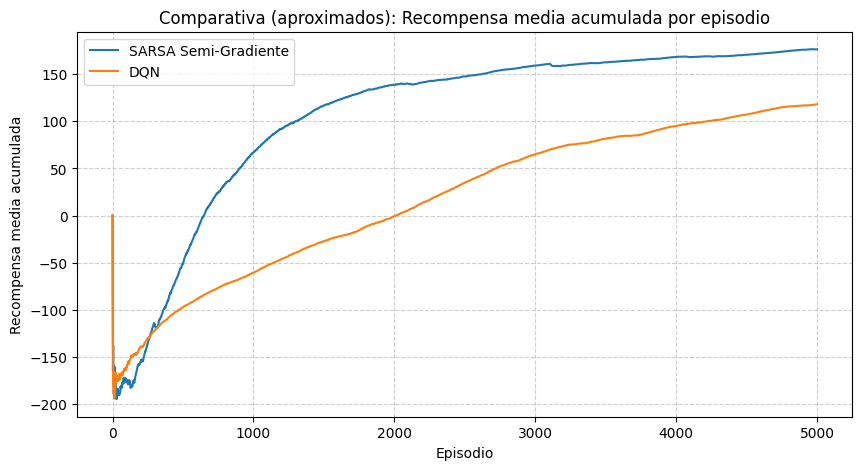
\includegraphics[width=0.9\linewidth]{imagenes/lunar_comparativa_recompensa.png}
    \caption{LunarLander-v3: recompensa media acumulada por episodio (SARSA-SG vs DQN).}
    \label{fig:lunar-comp-recompensa}
\end{figure}

\begin{figure}[!htbp]
    \centering
    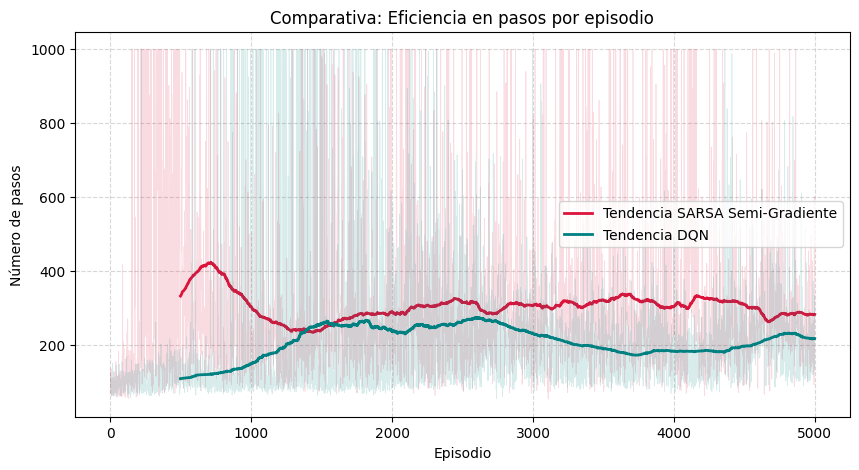
\includegraphics[width=0.9\linewidth]{imagenes/lunar_comparativa_pasos.png}
    \caption{LunarLander-v3: eficiencia en pasos por episodio (SARSA-SG vs DQN).}
    \label{fig:lunar-comp-pasos}
\end{figure}

\section{Conclusiones}

Los resultados permiten extraer varias conclusiones:
\begin{itemize}
    \item En entornos discretos largos (Taxi-v3), los métodos TD superan ampliamente a Monte Carlo por su bootstrapping paso a paso.
    \item La dimensión on-policy/off-policy es crítica en CliffWalking: SARSA aprende rutas seguras y Q-Learning tiende a la ruta óptima aunque explore con riesgo.
    \item En entornos continuos, la aproximación con redes es imprescindible. DQN es estable pero sensible a $C$ y al tamaño del buffer; SARSA-SG puede rendir mejor con una tasa de aprendizaje mayor.
    \item La comparación DQN vs SARSA-SG no es absoluta: el ranking depende de hiperparámetros y horizonte de entrenamiento.
\end{itemize}

Como trabajo futuro se propone repetir con múltiples semillas, igualar hiperparámetros entre aproximadores y evaluar variantes como Double DQN o Prioritized Replay.


% Bibliografía
\bibliographystyle{plain}
\bibliography{bibliography} % Si el archivo está en la carpeta docs


\end{document}